\section{Traces}
\label{qnodeos:sec:traces}

In our \ac{NV} experiments, the \ac{CNPU}, \ac{QNPU} and \ac{QDevice}, on both client and server nodes, trace (i.e. record the timestamps of) events happening on their system. The events that are traced on the \ac{CNPU} and \ac{QNPU} are listed in~\cref{tab:host_events,tab:qnpu_events}, respectively. The \ac{NV} \ac{QDevice} separately records messages received (physical instructions from the \ac{QNPU}, see~\cref{tab:qdevice-instructions}) and responses sent back to the \ac{QNPU}(see~\cref{tab:qdevice-return-values}).

\Cref{fig:delcomp-trace-example} shows a full-stack trace slice of a single execution of the \ac{DQC} circuit. This particular sequence of events started at offset 60460\,ms from the start of the experiment. The following events (among others) can be seen:
%
\begin{itemize}
    \item At $\approx$\,60470\,ms: client \ac{CNPU} sends subroutine C1 to the \ac{QNPU}; it is received slightly after on the \ac{QNPU} (\texttt{PROCMGR\_SUBROUTINE\_ADDED\_P0}).
    \item Slightly after 60470\,ms: the \ac{QNPU} starts the user process containing C1; it hits the entanglement instruction and moves the process to the waiting state (\texttt{PROCESSOR\_WAIT\_USER\_PROCESS}).
    \item At 60480\,ms: the first next time bin starts, starting the network process on both client and server. This results in \texttt{ENTANGLE} commands being sent to the \acp{QDevice} by both client and server.
    \item Between 60480 and 60550\,ms: the two \acp{QDevice} repeatedly attempt entanglement but fail (each \texttt{ENTANGLE} instruction from the \ac{QNPU} starts one batch; each \texttt{ENTANGLEMENT\_FAILURE} return message indicates the batch failed).
    \item Meanwhile at 60485\,ms, the server \ac{CNPU} sends subroutine S1 to the \ac{QNPU}.
    \item At $\approx$\,60552.5\,ms, the \acp{QDevice} succeed in entanglement generation, producing a $\ket{\Psi^+}$ Bell pair.
    \item After this, the client and server finish C1 and S1, respectively. The client sends instructions for local gates ending with a \texttt{MEASURE} physical instruction. The server starts S1, hits the \texttt{recv\_epr} instruction, goes into the waiting state, gets immediately unblocked (since the entangled pair was already created) and sends a bell state correction gate to the \ac{QDevice} (\texttt{X180}).
    \item At $\approx$\,60553.5\,ms, the client \ac{CNPU} receives the result of C1 (\texttt{RESULT\_RCVD}), and sends the classical message $\delta$ to the server \ac{CNPU} (\texttt{CLAS\_MSG\_SENT}).
    \item At $\approx$\,60554\,ms, the server \ac{CNPU} receives $\delta$ (\texttt{CLAS\_MSG\_RCVD}).
    \item At $\approx$\,60557\,ms, the server \ac{CNPU} sends S2 to the \ac{QNPU}. The \ac{QNPU} executes the user process containing S2 which involves sending local quantum instructions to the \ac{QDevice} ending with a measurement.
    \item At $\approx$\,60558\,ms, the \ac{QNPU} sends the result of S2 to the \ac{CNPU}.
\end{itemize}

\clearpage

\begin{table*}[htpb]
    \centering
    \begin{tabular}{|c|l|}
    \hline
    \textbf{Event name} & \textbf{Description} \\ 
    \hline
    \texttt{SUBROUTINE\_SEND\_ATTEMPT} & Try to send subroutine to \ac{QNPU} \\
    \texttt{SUBROUTINE\_SENT} & Subroutine sent to \ac{QNPU} \\ 
    \texttt{RESULT\_RCVD} & Subroutine results received from \ac{QNPU} \\
    \texttt{CLAS\_MSG\_SENT} & Classical message sent to other node \\
    \texttt{CLAS\_MSG\_RCVD} & Classical message received from other node \\
    \hline
    \end{tabular}
    \caption{\ac{CNPU} events that are traced (recorded with their timestamps) during application execution.}
    \label{tab:host_events}
\end{table*}

\begin{table*}[htpb]
    \centering
    \begin{tabular}{|c|l|}
    \hline
    \textbf{Event name} & \textbf{Description} \\ 
    \hline
    \texttt{SCHEDULER\_ARRIVE\_USER\_PROCESS} & A user process goes to the Ready state \\
    \texttt{SCHEDULER\_SCHEDULE\_USER\_PROCESS} & A user process goes to the Running state \\
    \texttt{SCHEDULER\_ARRIVE\_NET\_PROCESS} & Network process goes to the Ready state \\
    \texttt{SCHEDULER\_SCHEDULE\_NET\_PROCESS} & Network process goes to the Running state \\
    \texttt{PROCMGR\_SUBROUTINE\_ADDED\_P<i>} & New subroutine received from \ac{CNPU} for process <i> \\
    \texttt{PROCMGR\_SUBROUTINE\_DONE\_P<i>} & A subroutine for process <i> finished execution \\
    \texttt{PROCESSOR\_START\_USER\_PROCESS} & Processor starts or resumes executing a user process \\
    \texttt{PROCESSOR\_WAIT\_USER\_PROCESS} & Processor suspends a user process and puts it in the Waiting state \\
    \texttt{PROCESSOR\_FINISH\_USER\_PROCESS} & Processor stops executing a user process \\
    \texttt{PROCESSOR\_START\_NET\_PROCESS} & Processor starts or resumes executing the network process \\
    \texttt{PROCESSOR\_FINISH\_NET\_PROCESS} & Processor stops executing the network process \\
    \texttt{QDEVICE\_PRODUCE\_<cmd>\_CMD} & Processor prepares <cmd> command for the \ac{QDevice} \\
    \texttt{QDEVICE\_CONSUME\_CMD} & \ac{QDevice} reads the next command from the \ac{QNPU} \\
    \texttt{QDEVICE\_PRODUCE\_OUTCOME} & \ac{QDevice} sends result to the \ac{QNPU} \\
    \texttt{PROCESSOR\_CONSUME\_OUTCOME} & Processor reads \ac{QDevice} result \\
    \texttt{QNETWORK\_ENT\_PULL} & Network stack pulls instruction from the EGP \\
    \texttt{EGP\_NEI\_OK} & QEGP notifies that EPR pair has been created \\
    \hline
    \end{tabular}
    \caption{\ac{QNPU} events that are traced (recorded with their timestamps) during application execution. <i> can be any number from 0 to 9 (`subroutine added` and `subroutine done` events are not traced for processes with ID 10 or larger). <cmd> can be any physical instruction.}
    \label{tab:qnpu_events}
\end{table*}

\begin{figure*}
\centering
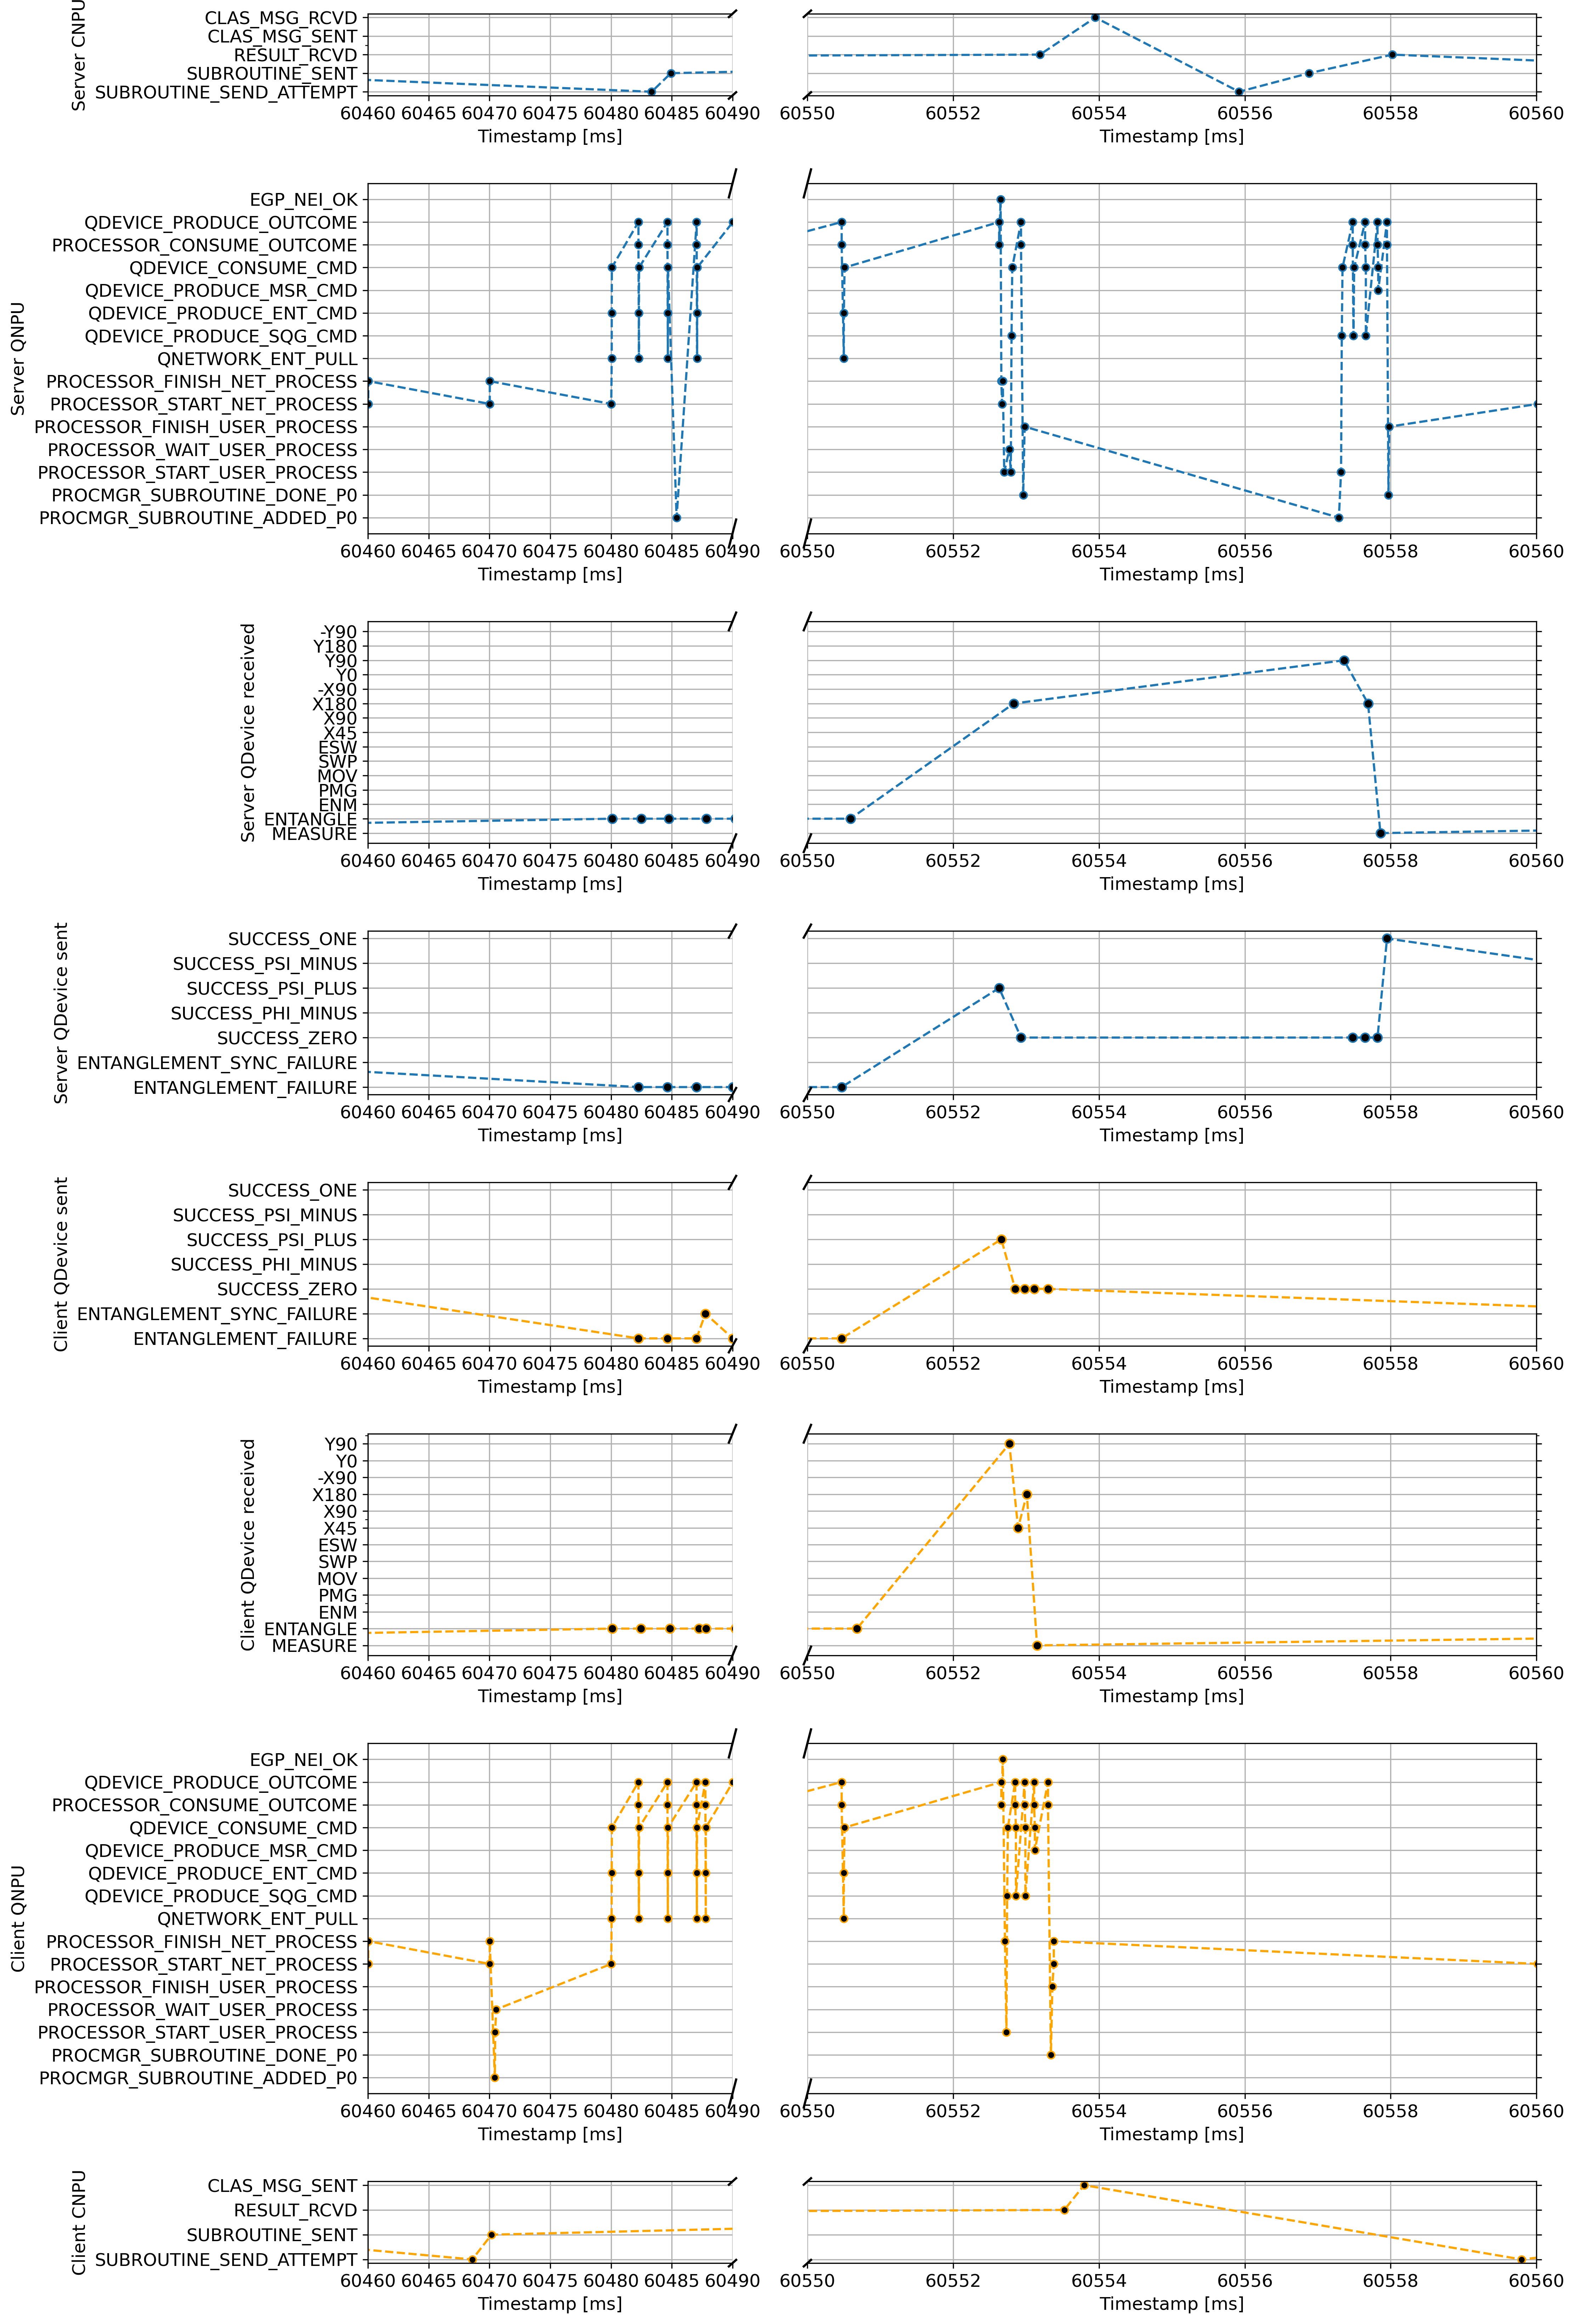
\includegraphics[width=0.8\linewidth]{figures/qnodeos/supplementary/plots/full_slice.png}
\caption{Full-stack event trace for one particular execution of the \ac{DQC} circuit. Between timestamps 60490 and 60550 are more entanglement attempts which are cut out for the sake of clarity.}
\label{fig:delcomp-trace-example}
\end{figure*}
